\documentclass[12pt,]{article}
\usepackage{lmodern}
\usepackage{amssymb,amsmath}
\usepackage{ifxetex,ifluatex}
\usepackage{fixltx2e} % provides \textsubscript
\ifnum 0\ifxetex 1\fi\ifluatex 1\fi=0 % if pdftex
  \usepackage[T1]{fontenc}
  \usepackage[utf8]{inputenc}
\else % if luatex or xelatex
  \ifxetex
    \usepackage{mathspec}
    \usepackage{xltxtra,xunicode}
  \else
    \usepackage{fontspec}
  \fi
  \defaultfontfeatures{Mapping=tex-text,Scale=MatchLowercase}
  \newcommand{\euro}{€}
\fi
% use upquote if available, for straight quotes in verbatim environments
\IfFileExists{upquote.sty}{\usepackage{upquote}}{}
% use microtype if available
\IfFileExists{microtype.sty}{%
\usepackage{microtype}
\UseMicrotypeSet[protrusion]{basicmath} % disable protrusion for tt fonts
}{}
\usepackage[margin=1in]{geometry}
\usepackage{longtable,booktabs}
\usepackage{graphicx}
\makeatletter
\def\maxwidth{\ifdim\Gin@nat@width>\linewidth\linewidth\else\Gin@nat@width\fi}
\def\maxheight{\ifdim\Gin@nat@height>\textheight\textheight\else\Gin@nat@height\fi}
\makeatother
% Scale images if necessary, so that they will not overflow the page
% margins by default, and it is still possible to overwrite the defaults
% using explicit options in \includegraphics[width, height, ...]{}
\setkeys{Gin}{width=\maxwidth,height=\maxheight,keepaspectratio}
\ifxetex
  \usepackage[setpagesize=false, % page size defined by xetex
              unicode=false, % unicode breaks when used with xetex
              xetex]{hyperref}
\else
  \usepackage[unicode=true]{hyperref}
\fi
\hypersetup{breaklinks=true,
            bookmarks=true,
            pdfauthor={},
            pdftitle={Stock Assessment of China Rockfish in 2015},
            colorlinks=true,
            citecolor=blue,
            urlcolor=blue,
            linkcolor=magenta,
            pdfborder={0 0 0}}
\urlstyle{same}  % don't use monospace font for urls
\setlength{\parindent}{0pt}
\setlength{\parskip}{6pt plus 2pt minus 1pt}
\setlength{\emergencystretch}{3em}  % prevent overfull lines
\setcounter{secnumdepth}{5}

%%% Use protect on footnotes to avoid problems with footnotes in titles
\let\rmarkdownfootnote\footnote%
\def\footnote{\protect\rmarkdownfootnote}

%%% Change title format to be more compact
\usepackage{titling}
\setlength{\droptitle}{-2em}
  \title{Stock Assessment of China Rockfish in 2015}
  \pretitle{\vspace{\droptitle}\centering\huge}
  \posttitle{\par}
  \author{}
  \preauthor{}\postauthor{}
  \date{}
  \predate{}\postdate{}


\usepackage{fullpage}
\usepackage{booktabs}
\usepackage{tabularx}
\usepackage{longtable}
\usepackage{multirow}
\usepackage{multicol}
\usepackage{rotating}
\usepackage{lscape}
\usepackage{threeparttablex}
\usepackage{appendix}
\usepackage{wrapfig}
\usepackage{array}
\usepackage{pdfpages}
\usepackage{lineno}
%\usepackage[inline]{showlabels} % remove for final
\usepackage[singlelinecheck=off]{caption}   % remove for final
\usepackage{float}
\usepackage{placeins} % keeps floats from moving
\usepackage{draftwatermark}
\usepackage{authblk}
\usepackage{caption}
\usepackage{fancyhdr}
\usepackage{appendix}
\usepackage{indentfirst} % indents first paragraph of a section
\usepackage{mdwtab}
\usepackage{subfigure} % continued float multi-page figure
\usepackage{enumerate} % for lists
\usepackage{hyperref}
\hypersetup{colorlinks=true, urlcolor=blue, linktoc=page, linkcolor=blue, citecolor=blue}
\usepackage{array}
\usepackage{graphicx}
\usepackage[space]{grffile}   %spaces in file name path


\begin{document}

\maketitle



\begin{center}
\thispagestyle{empty}

\vspace{2cm}

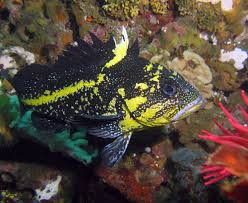
\includegraphics{chinarockfish}~\\[1cm]



E.J. Dick\textsuperscript{1}\\
Melissa Monk\textsuperscript{1}\\
Ian Taylor\textsuperscript{2}\\
Melissa Haltuch\textsuperscript{2}\\

\vspace{1cm}


\textsuperscript{1}Southwest Fisheries Science Center, U.S. Department of Commerce, National Oceanic and Atmospheric Administration, National Marine Fisheries Service, 110 Shaffer Road, Santa Cruz, California 95060\\

\textsuperscript{2}Northwest Fisheries Science Center, U.S. Department of Commerce, National Oceanic and Atmospheric Administration,National Marine Fisheries Service, 2725 Montlake Boulevard East, Seattle, Washington 98112\\

\vfill
\textsc{\Large DRAFT SAFE}\\[0.5cm]
%Bottom of the page
{\large \today}

\maketitle

\pagenumbering{roman}
\setcounter{page}{1}
\end{center}

{
\hypersetup{linkcolor=black}
\setcounter{tocdepth}{4}
\tableofcontents
}
\pagebreak
\pagenumbering{arabic} \setcounter{page}{1}

\section*{Executive summary}\label{executive-summary}
\addcontentsline{toc}{section}{Executive summary}

adfadfaf

\subsection*{Stock}\label{stock}
\addcontentsline{toc}{subsection}{Stock}

Blah blah Milton says China rockfish live to at least 79 years (Love et
al. 2002).

\subsection*{Catches}\label{catches}
\addcontentsline{toc}{subsection}{Catches}

Trends and current levels-include table for last ten years and graph
with long term data

\begin{table}[ht]
\centering
\caption{Recent trend in beginning of the year biomass and depletion} 
\label{SpawningB}
\begin{tabularx}{\textwidth}{l>{\centering}p{1in}>{\centering}p{1.2in}}
  \hline
Year & Spawning Biomass (mt) & \~{} 95\% confidence interval \\ 
  \hline
2004 & 1760 & (478-3043) \\ 
  2005 & 1727 & (445-3010) \\ 
  2006 & 1710 & (427-2994) \\ 
  2007 & 1695 & (409-2980) \\ 
  2008 & 1680 & (392-2969) \\ 
  2009 & 1672 & (378-2965) \\ 
  2010 & 1659 & (359-2960) \\ 
  2011 & 1660 & (352-2968) \\ 
  2012 & 1669 & (353-2985) \\ 
  2013 & 1673 & (348-2998) \\ 
   \hline
\end{tabularx}
\end{table}

\subsection*{Data and assessment}\label{data-and-assessment}
\addcontentsline{toc}{subsection}{Data and assessment}

date of last assessment, type of assessment model, data available, new
information, and information lacking

\subsection*{Stock biomass}\label{stock-biomass}
\addcontentsline{toc}{subsection}{Stock biomass}

trends and current levels relative to virgin or historic levels,
description of uncertainty-include table for last 10 years and graph
with long term estimates

\begin{figure}[htbp]
\centering
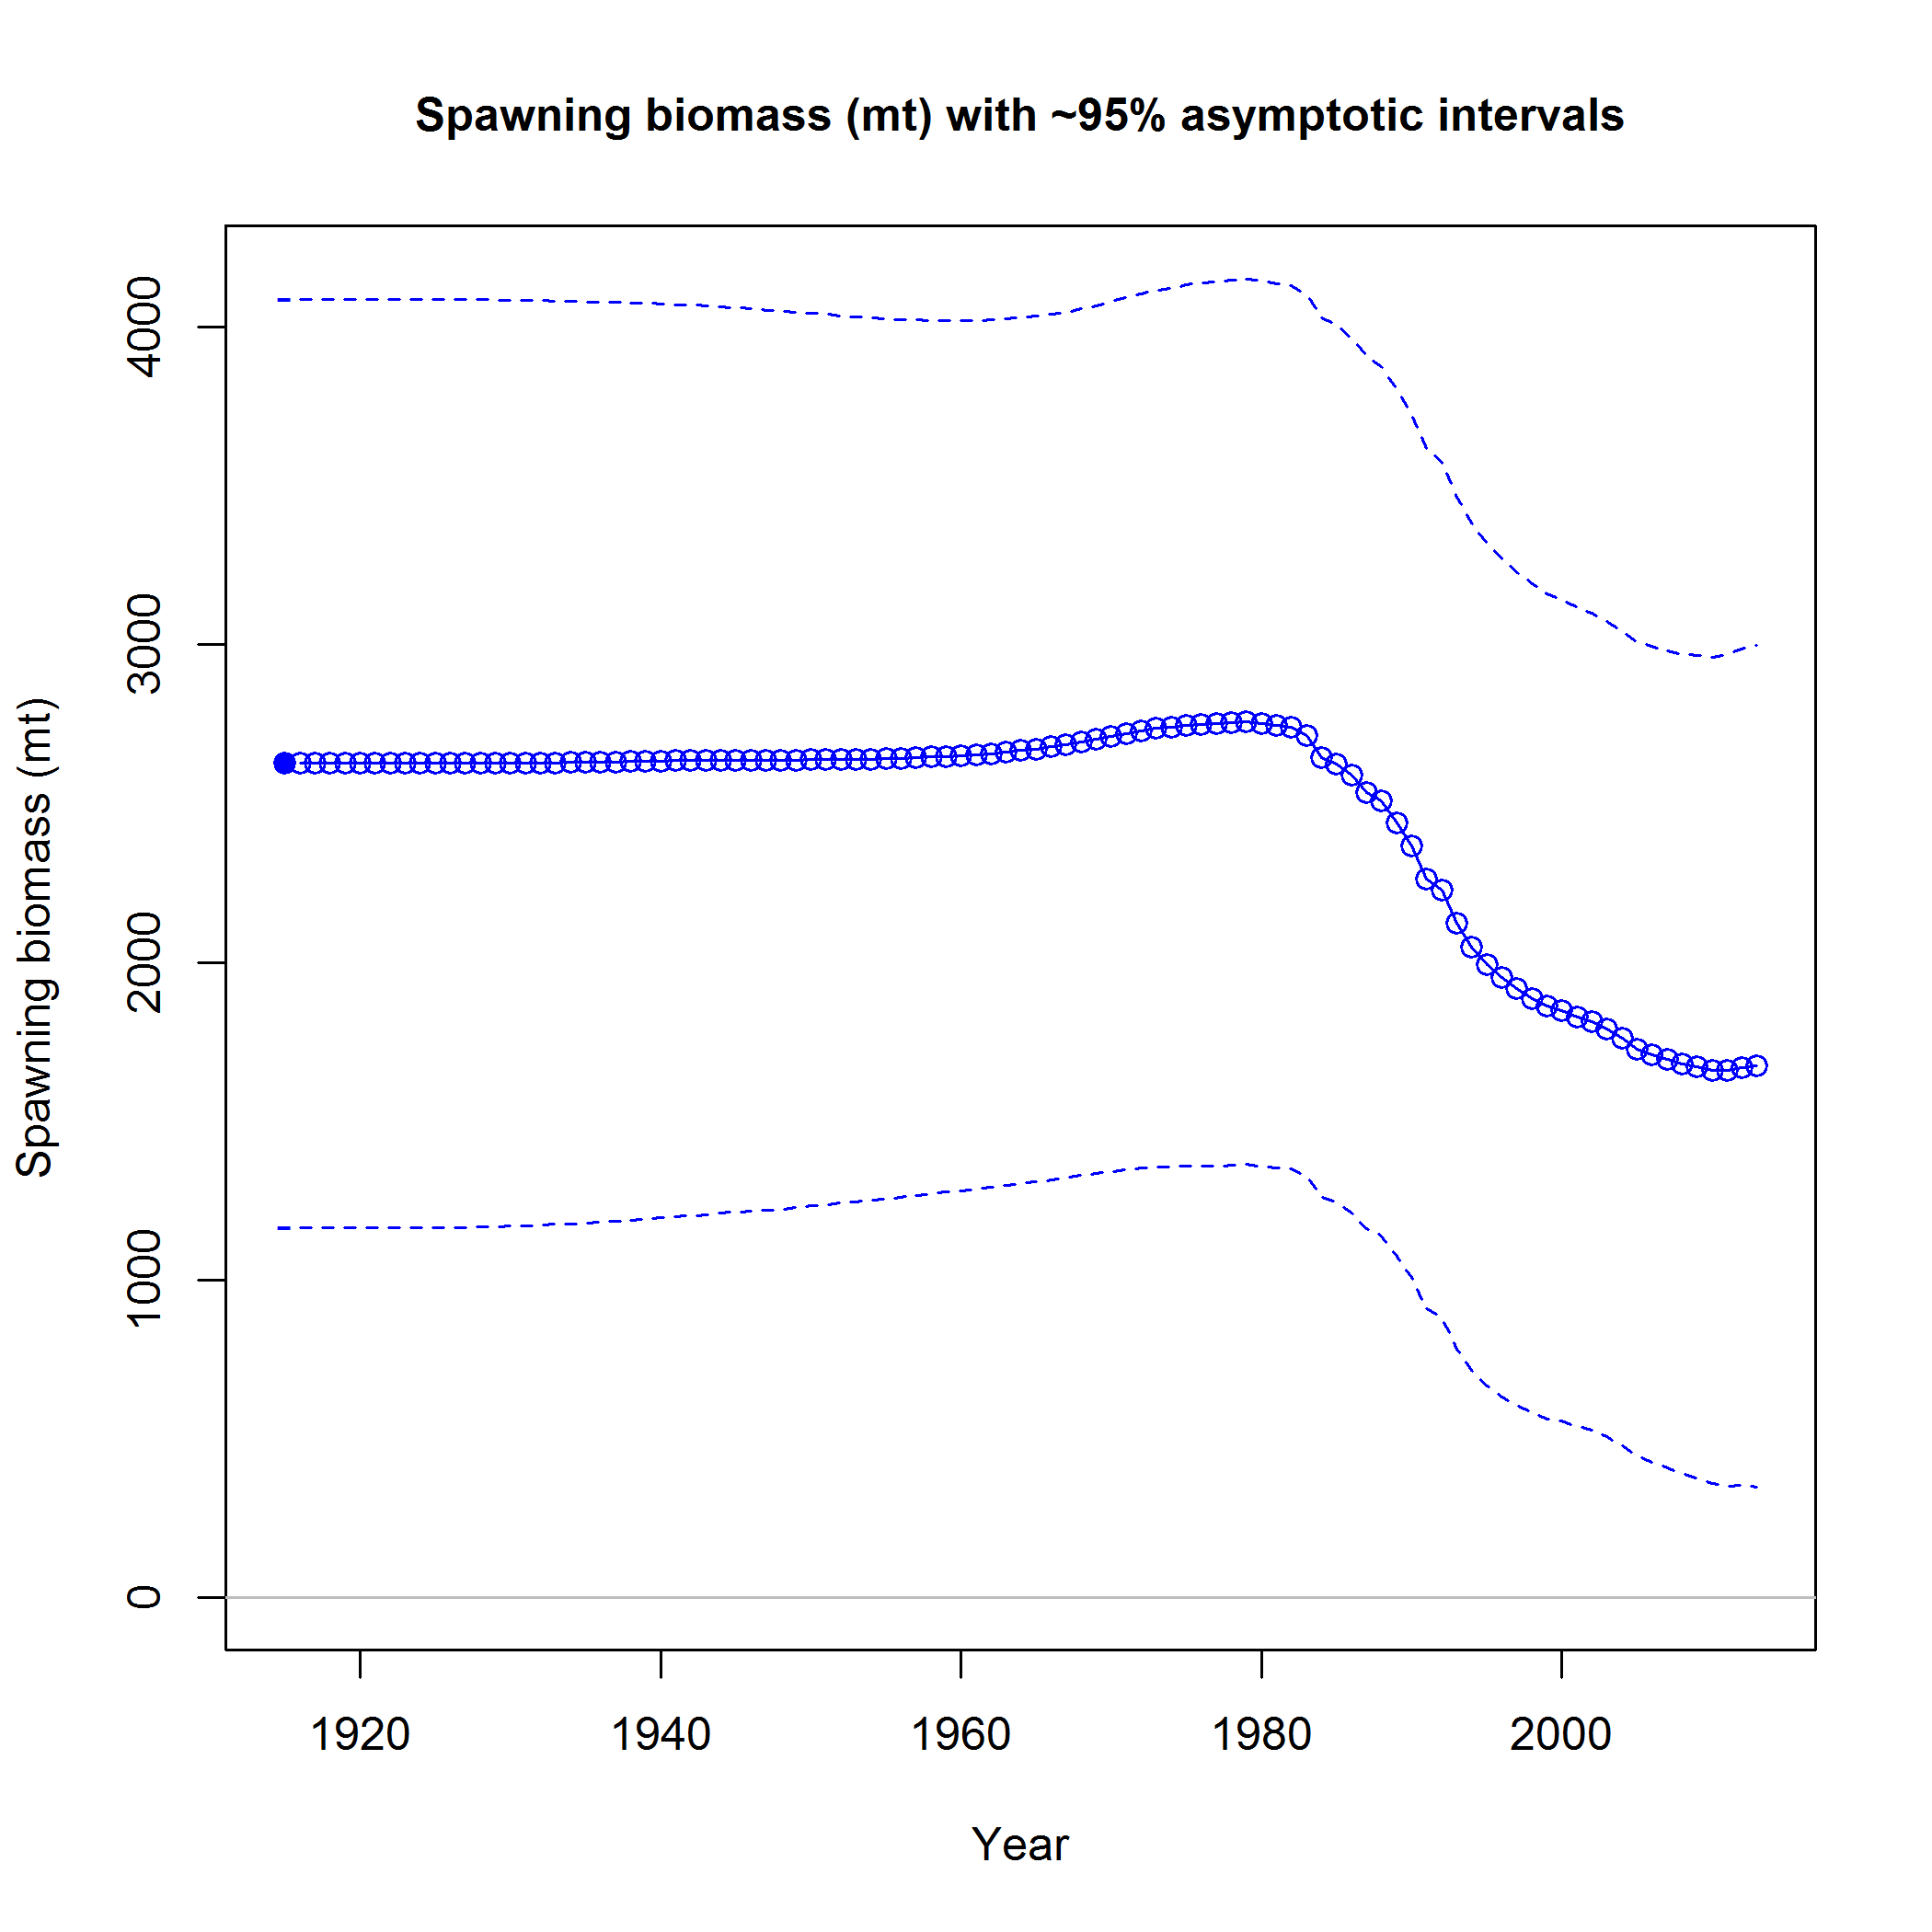
\includegraphics{plots/spawningB.png}
\caption{Time series of spawning biomass trajectory (circles and line:
median; light broken lines: 95\% credibility intervals) for China
rockfish. \label{spawningB}}
\end{figure}

This is a test to see if I can reference Figure \ref{spawningB}.

\subsection*{Recruitment}\label{recruitment}
\addcontentsline{toc}{subsection}{Recruitment}

trends and current levels relative to virgin or historic levels-include
table for last 10 years and graph with long term estimates

\subsection*{Exploitation status}\label{exploitation-status}
\addcontentsline{toc}{subsection}{Exploitation status}

exploitation rates, i.e., total catch divided by exploitable biomass, or
the annual SPR harvest rate - include a table with the last 10 years of
data and a graph showing the trend in fishing mortality relative to the
target (y-axis) plotted against the trend in biomass relative to the
target (x-axis).

\subsection*{Ecosystem considerations}\label{ecosystem-considerations}
\addcontentsline{toc}{subsection}{Ecosystem considerations}

\subsection*{Reference points (groundfish)/harvest control rules
(CPS)}\label{reference-points-groundfishharvest-control-rules-cps}
\addcontentsline{toc}{subsection}{Reference points (groundfish)/harvest
control rules (CPS)}

management targets and definition of overfishing, including the harvest
rate that brings the stock to equilibrium at B40\% (the BMSY proxy) and
the equilibrium stock size that results from fishing at the default
harvest rate (the FMSY proxy). Include a summary table that compares
estimated reference points for SSB, SPR, Exploitation Rate and Yield
based on SSBproxy for MSY, SPRproxy for MSY, and estimated MSY values
(table i. on page 35 of attached Canary rockfish executive summary).

\subsection*{Management performance}\label{management-performance}
\addcontentsline{toc}{subsection}{Management performance}

catches in comparison to OFL, ABC and OY/ACL values for the most recent
10 years (when available), overfishing levels, actual catch and discard.
Include OFL(encountered), OFL(retained) and OFL(dead) if different due
to discard and discard mortality.

\subsection*{Unresolved problem and major
uncertainties}\label{unresolved-problem-and-major-uncertainties}
\addcontentsline{toc}{subsection}{Unresolved problem and major
uncertainties}

any special issues that complicate scientific assessment, questions
about the best model scenario, etc.

\subsection*{Decision table (groundfish
only)*}\label{decision-table-groundfish-only}
\addcontentsline{toc}{subsection}{Decision table (groundfish only)*}

projected yields (OFL, ABC and ACL), spawning biomass, and stock
depletion levels for each year.* (Not required in draft assessments
undergoing review.)

\subsection*{Research and data needs}\label{research-and-data-needs}
\addcontentsline{toc}{subsection}{Research and data needs}

identify information gaps that seriously impede the stock assessment.

\subsection*{Rebuilding projections}\label{rebuilding-projections}
\addcontentsline{toc}{subsection}{Rebuilding projections}

reference to the principal results from rebuilding analysis if the stock
is overfished.* This section should be included in the Final/SAFE
version assessment document but is not required for draft assessments
undergoing review. See Rebuilding Analysis terms of reference for
detailed information on rebuilding analysis requirements.

\section{Introduction}\label{introduction}

\subsection{Basic Information}\label{basic-information}

Scientific name, distribution, the basis of the choice of stock
structure, including regional differences in life history or other
biological characteristics that should form the basis of management
units.

\subsection{Map}\label{map}

A map showing the scope of the assessment and depicting boundaries for
fisheries or data collection strata.

\subsection{Life History}\label{life-history}

Important features of life history that affect management (e.g.,
migration, sexual dimorphism, bathymetric demography).

\subsection{Ecosysem Considerations}\label{ecosysem-considerations}

Ecosystem considerations (e.g., ecosystem role and trophic relationships
of the species, habitat requirements/preferences, relevant data on
ecosystem processes that may affect stock or parameters used in the
stock assessment, and/or cross-FMP interactions with other fisheries).
This section should note if environmental correlations or food web
interactions were incorporated into the assessment model. The length and
depth of this section would depend on availability of data and reports
from the IEA, expertise of the STAT, and whether ecosystem factors are
informational to contribute quantitative information to the assessment.

\subsection{Fishery Information}\label{fishery-information}

Important features of current fishery and relevant history of fishery.

\subsection{Summary of Management
History}\label{summary-of-management-history}

Summary of management history (e.g., changes in mesh sizes, trip limits,
or other management actions that may have significantly altered
selection, catch rates, or discards).

\subsection{Managament Performance}\label{managament-performance}

Management performance, including a table or tables comparing
Overfishing Limit (OFL), Annual Catch Limit (ACL), Harvest Guideline
(HG) {[}CPS only{]}, landings, and catch (i.e., landings plus discard)
for each area and year

\subsection{Fisheries off Canada, Alaska, and/or
Mexico}\label{fisheries-off-canada-alaska-andor-mexico}

Description of fisheries for this species off Canada, Alaska and/or
Mexico, including references to any recent assessments of those stocks.

\section{Assessment}\label{assessment}

\subsection{Data}\label{data}

\subsubsection{Title}\label{title}

Landings by year and fishery, historical catch estimates, discards
(generally specified as a percentage of total catch in weight and in
units of mt), catch-at-age, weight-at-age, abundance indices (typically
survey and CPUE data), data used to estimate biological parameters
(e.g., growth rates, maturity schedules, and natural mortality) with
coefficients of variation (CVs) or variances if available. Include
complete tables and figures and date of extraction.

\subsubsection{Title}\label{title-1}

Sample size information for length and age composition data by area,
year, gear, market category, etc., including both the number of trips
and fish sampled.

\subsubsection{Title}\label{title-2}

All data sources that include the species being assessed, which are used
in the assessment, and provide the rationale for data sources that are
excluded.

\subsubsection{Title}\label{title-3}

Clear description of environmental or ecosystem data if included in the
assessment.

\subsection{History of Modeling Approaches Used for this
Stock}\label{history-of-modeling-approaches-used-for-this-stock}

\subsubsection{Title}\label{title-4}

Response to STAR panel recommendations from the most recent previous
assessment.

\subsubsection{Title}\label{title-5}

Report of consultations with AP and MT representatives regarding the use
of various data sources in the stock assessment.

\subsubsection{Title}\label{title-6}

If environmental or ecosystem data are incorporated, report of
consultations with technical teams that evaluated ecosystem data or
methodologies used in the assessment.

\subsection{Model Description}\label{model-description}

\subsubsection{Title}\label{title-7}

Complete description of any new modeling approaches.

\subsubsection{Title}\label{title-8}

Definitions of fleets and areas.

\subsubsection{Title}\label{title-9}

Assessment program with last revision date (i.e., date executable
program file was compiled).

\subsubsection{Title}\label{title-10}

List and description of all likelihood components in the model

\subsubsection{Title}\label{title-11}

Constraints on parameters, selectivity assumptions, natural mortality,
treatment of age reading bias and/or imprecision, and other fixed
parameters.

\subsubsection{Title}\label{title-12}

Description of stock-recruitment constraints or components.

\subsubsection{Title}\label{title-13}

Description of how the first year that is included in the model was
selected and how the population state at the time is defined (e.g., B0,
stable age structure, etc.).

\subsubsection{Title}\label{title-14}

Critical assumptions and consequences of assumption failures.

\subsection{Model Selection and
Evaluation}\label{model-selection-and-evaluation}

\subsubsection{Title}\label{title-15}

Evidence of search for balance between model realism and parsimony.

\subsubsection{Title}\label{title-16}

Comparison of key model assumptions, include comparisons based on nested
models (e.g., asymptotic vs.~domed selectivities, constant
vs.~time-varying selectivities).

\subsubsection{Title}\label{title-17}

Summary of alternate model configurations that were tried but rejected.

\subsubsection{Title}\label{title-18}

Likelihood profile for the base-run (or proposed base-run model for a
draft assessment undergoing review) configuration over one or more key
parameters (e.g., M, h, Q) to show consistency among input data sources.

\subsubsection{Title}\label{title-19}

Residual analysis for the base-run configuration (or proposed base-run
model in a draft assessment undergoing review) e.g., residual plots,
time series plots of observed and predicted values, or other approaches.
Note that model diagnostics are required in draft assessments undergoing
review.

\subsubsection{Title}\label{title-20}

Convergence status and convergence criteria for the base-run model (or
proposed base run).

\subsubsection{Title}\label{title-21}

Randomization run results or other evidence of search for global best
estimates.

\subsubsection{Title}\label{title-22}

Evaluation of model parameters. Do they make sense? Are they credible?

\subsubsection{Title}\label{title-23}

Are model results consistent with assessments of the same species in
Canada and Alaska? Are parameter estimates (e.g., survey catchability)
consistent with estimates for related stocks?

\subsection{Response to STAR Panel
Recommendations}\label{response-to-star-panel-recommendations}

Point-by-point response to the STAR panel recommendations

\subsection{Base-Model(s) Results}\label{base-models-results}

\subsubsection{Title}\label{title-24}

Table listing all explicit parameters in the stock assessment model used
for base model, their purpose (e.g., recruitment parameter, selectivity
parameter) and whether or not the parameter was actually estimated in
the stock assessment model.

\subsubsection{Title}\label{title-25}

Population numbers at age × year × sex (if sex-specific M, growth, or
selectivity) (May be provided as a text or spreadsheet file).* Not
required in draft assessment undergoing review.

\subsubsection{Title}\label{title-26}

Time-series of total, 1+ (if age 1s are in the model), summary, and
spawning biomass (and/or spawning output), depletion relative to B0,
recruitment and fishing mortality or exploitation rate estimates (table
and figures).

\subsubsection{Title}\label{title-27}

Selectivity estimates (if not included elsewhere).

\subsubsection{Title}\label{title-28}

Stock-recruitment relationship.

\subsubsection{Title}\label{title-29}

OFL, ABC and ACL (and/or ABC and OY or HG) for recent years.

\subsubsection{Title}\label{title-30}

Clear description of units for all outputs.

\subsubsection{Title}\label{title-31}

Clear description of how discard is included in yield estimates.

\subsubsection{Title}\label{title-32}

Clear description of environmental or ecosystem data if included in the
assessment.

\subsection{Uncertainty and Sensitivity
Analyses}\label{uncertainty-and-sensitivity-analyses}

\label{sec:uncertainty} The best approach for describing uncertainty and
the range of probable biomass estimates in groundfish assessments may
depend on the situation.\\Important factors to consider include:

\subsubsection{Title}\label{title-33}

Parameter uncertainty (variance estimation conditioned on a given model,
estimation framework, data set choice, and weighting scheme), including
likelihood profiles for important assessment parameters (e.g., natural
mortality). This also includes expressing uncertainty in derived outputs
of the model and estimating CVs using appropriate methods (e.g.,
bootstrap, asymptotic methods, Bayesian approaches, such as MCMC).
Include the CV of spawning biomass in the first year for which an OFL
has not been specified (typically end year +1 or +2).

\subsubsection{Title}\label{title-34}

Sensitivity to assumptions about model structure, i.e., model
specification uncertainty

\subsubsection{Title}\label{title-35}

Sensitivity to data set choice and weighting schemes (e.g., emphasis
factors), which may also include a consideration of recent patterns in
recruitment.

\subsubsection{Title}\label{title-36}

Retrospective analysis, where the model is fitted to a series of
shortened input data sets, with the most recent years of input data
being dropped.

\subsubsection{Title}\label{title-37}

Historical analysis (plot of actual estimates from current and previous
assessments).

\subsubsection{Title}\label{title-38}

Subjective appraisal of the magnitude and sources of uncertainty.

\subsubsection{Title}\label{title-39}

If a range of model runs is used to characterize uncertainty it is
important to provide some qualitative or quantitative information about
relative probability of each. If no statements about relative
probability can be made, then it is important to state that all
scenarios (or all scenarios between the bounds depicted by the runs) are
equally likely

\subsubsection{Title}\label{title-40}

\label{sec:uncertaintylast} If possible, ranges depicting uncertainty
should include at least three runs: (a) one judged most probable; (b) at
least one that depicts the range of uncertainty in the direction of
lower current biomass levels; and (c) one that depicts the range of
uncertainty in the direction of higher current biomass levels. The
entire range of uncertainty should be carried through stock projections
and decision table analyses.

\section{Harvest Control Rules (CPS
Only)}\label{harvest-control-rules-cps-only}

\section{Reference Points (Groundfish
Only)}\label{reference-points-groundfish-only}

\begin{enumerate}
\def\labelenumi{\arabic{enumi}.}
\itemsep1pt\parskip0pt\parsep0pt
\item
  Unfished spawning stock biomass, summary age biomass, and recruitment,
  along with unfished spawning stock output.
\item
  Reference points based on B\textsubscript{40\%} for rockfish and
  roundfish and on B\textsubscript{25\%} for flatfish (spawning biomass
  and/or output, SPR, exploitation rate, equilibrium yield).
\item
  Reference points based on default SPR proxy (spawning biomass and/or
  output, SPR, exploitation rate, equilibrium yield).
\item
  Reference points based on MSY (if estimated) (spawning biomass and/or
  output, SPR, exploitation rate, equilibrium yield).
\item
  Equilibrium yield curve showing various BMSY proxies.
\end{enumerate}

\section{Harvest Projections and Decision Tables (Groundfish
Only)}\label{harvest-projections-and-decision-tables-groundfish-only}

*Not required in draft assessment undergoing review.

\begin{enumerate}
\def\labelenumi{\arabic{enumi}.}
\item
  Harvest projections and decision tables (i.e., a matrix of alternative
  models (states of nature) versus management actions) should cover the
  plausible range of uncertainty about current stock biomass and a set
  of candidate fishing mortality targets used for the stock. See section
  ``\textit{Uncertainty and Decision Tables in Groundfish Stock Assessment}''
  (this document, pp.
  \pageref{sec:uncertainty}-\pageref{sec:uncertaintylast}) on how to
  define alternative states of nature. Management decisions in most
  cases represent the sequence of catches including estimate of OFL
  based on FMSY (or its proxy) and those obtained by applying the
  Council 40-10 harvest policy to each state of nature; however other
  alternatives may be suggested by the GMT as being more relevant to
  Council decision making. OFL calculations should be based on the
  assumption that future catches equal ABCs and not OFLs.
\item
  Information presented should include biomass, stock depletion, and
  yield projections of OFL, ABC and ACL for ten years into the future,
  beginning with the first year for which management action could be
  based upon the assessment.
\end{enumerate}

\section{Regional Management
Considerations}\label{regional-management-considerations}

\begin{enumerate}
\def\labelenumi{\arabic{enumi}.}
\item
  For stocks where current practice is to allocate harvests by
  management area, a recommended method of allocating harvests based on
  the distribution of biomass should be provided. The MT advisor should
  be consulted on the appropriate management areas for each stock.
\item
  Discuss whether a regional management approach makes sense for the
  species from a biological perspective.
\item
  If there are insufficient data to analyze a regional management
  approach, what are the research and data needs to answer this
  question?
\end{enumerate}

\section{Research Needs}\label{research-needs}

\section{Acknowledgments}\label{acknowledgments}

Include STAR panel members and affiliations as well as names and
affiliations of persons who contributed data, advice or information but
were not part of the assessment team.
\textbf{* Not required in draft assessment undergoing review.}

\section{Tables}\label{tables}

\section{Figures}\label{figures}

\newpage

\section*{Appendix A. SS data file}\label{appendix-a.-ss-data-file}
\addcontentsline{toc}{section}{Appendix A. SS data file}

\renewcommand{\thepage}{A-\arabic{page}}
\renewcommand{\thefigure}{A\arabic{figure}}
\renewcommand{\thetable}{A\arabic{table}}

\setcounter{page}{1} \setcounter{figure}{1} \setcounter{table}{1}

Just writing something in here in reference to a fig \ref{appendfig}

\begin{figure}[htbp]
\centering
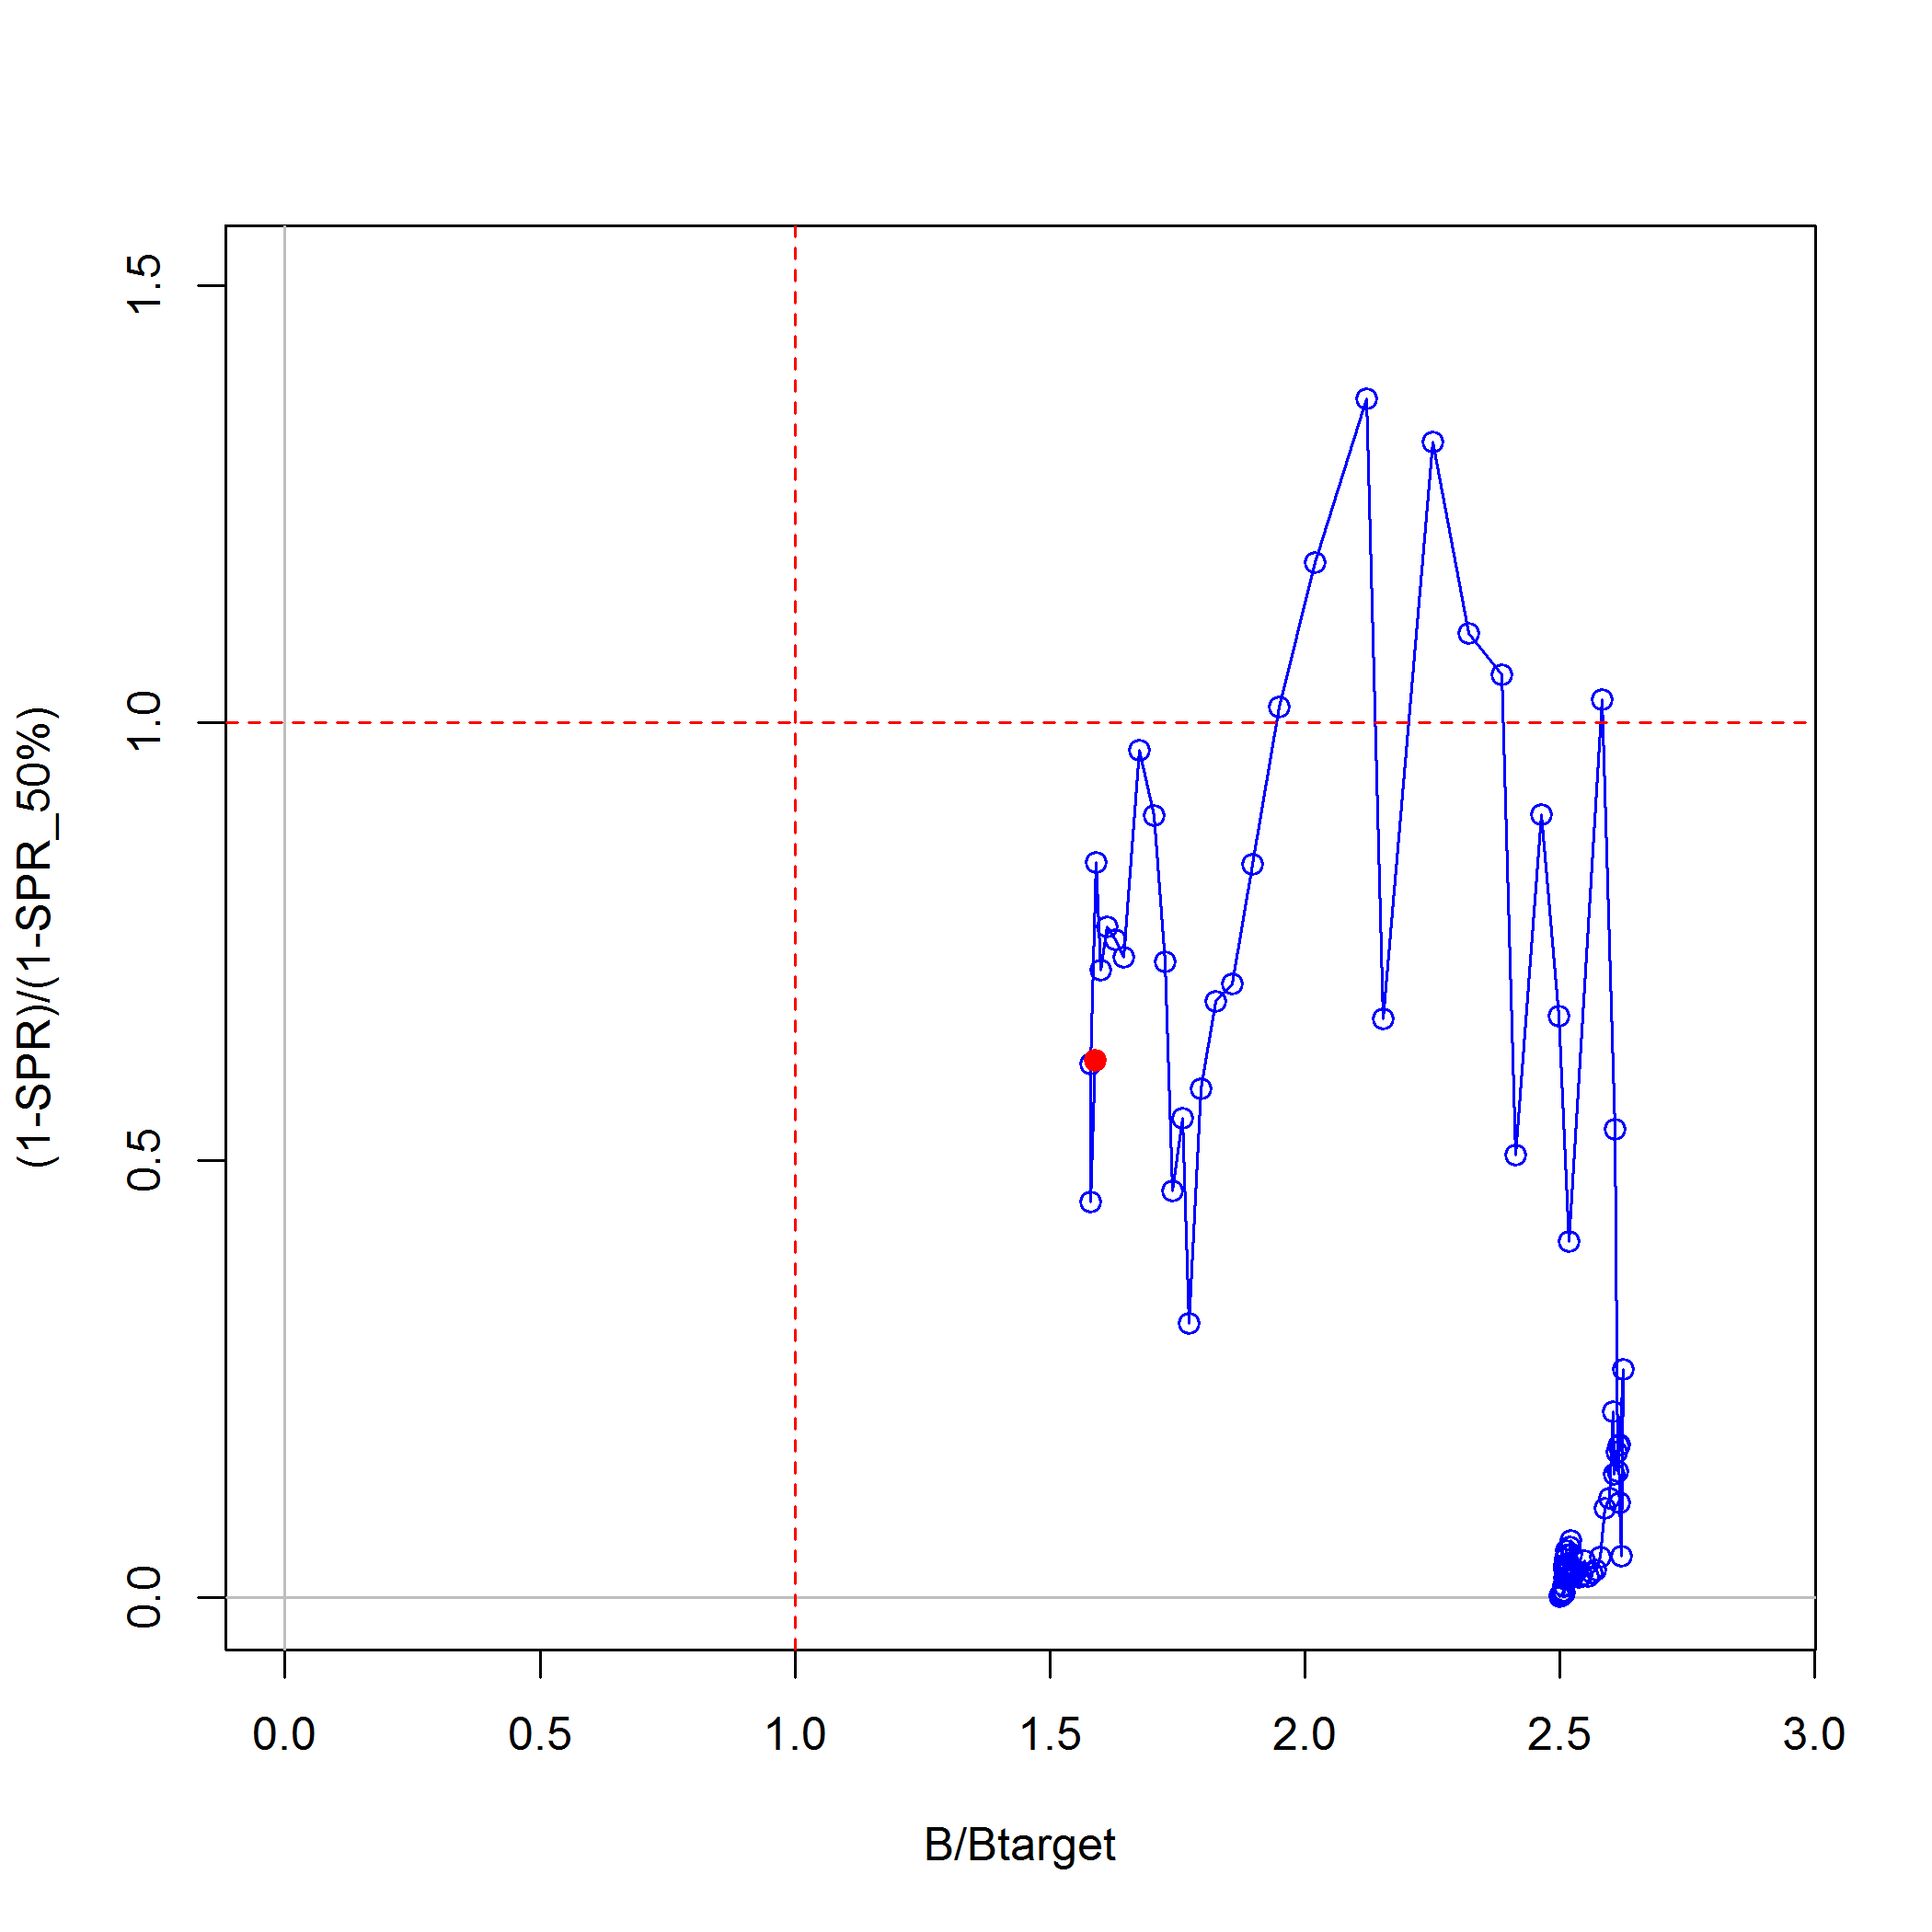
\includegraphics{plots/SPR4_phase}
\caption{appendix figure test \label{appendfig}}
\end{figure}

\newpage 

\subsection*{Appendix A1. Sub-headings in
Appendix}\label{appendix-a1.-sub-headings-in-appendix}
\addcontentsline{toc}{subsection}{Appendix A1. Sub-headings in Appendix}

\renewcommand{\thepage}{A1-\arabic{page}}
\renewcommand{\thefigure}{A1.\arabic{figure}}
\renewcommand{\thetable}{A1.\arabic{table}}

\setcounter{page}{1} \setcounter{figure}{1} \setcounter{table}{1}

\newpage

\section*{Appendix B. SS control
file}\label{appendix-b.-ss-control-file}
\addcontentsline{toc}{section}{Appendix B. SS control file}

\renewcommand{\thepage}{B-\arabic{page}}
\renewcommand{\thefigure}{B\arabic{figure}}
\renewcommand{\thetable}{B\arabic{table}}

\setcounter{page}{1} \setcounter{figure}{1} \setcounter{table}{1}

\newpage

\section*{Appendix C. SS starter
file}\label{appendix-c.-ss-starter-file}
\addcontentsline{toc}{section}{Appendix C. SS starter file}

\renewcommand{\thepage}{C-\arabic{page}}
\renewcommand{\thefigure}{C\arabic{figure}}
\renewcommand{\thetable}{C\arabic{table}}

\setcounter{page}{1} \setcounter{figure}{1} \setcounter{table}{1}

\newpage

\section*{Appendix D. SS forecast
file}\label{appendix-d.-ss-forecast-file}
\addcontentsline{toc}{section}{Appendix D. SS forecast file}

\renewcommand{\thepage}{D-\arabic{page}}
\renewcommand{\thefigure}{D\arabic{figure}}
\renewcommand{\thetable}{D\arabic{table}}

\setcounter{page}{1} \setcounter{figure}{1} \setcounter{table}{1}

\newpage

\section*{Appendix E. Observed Angler
Prediction}\label{appendix-e.-observed-angler-prediction}
\addcontentsline{toc}{section}{Appendix E. Observed Angler Prediction}

\renewcommand{\thepage}{E-\arabic{page}}
\renewcommand{\thefigure}{E\arabic{figure}}
\renewcommand{\thetable}{E\arabic{table}}

\setcounter{page}{1} \setcounter{figure}{1} \setcounter{table}{1}

Beginning in 1992 Calrec Historic began tracking the number of observed
anglers in its database, however the full data-set spans from 4/22/87
until 12/31/98. The goal of this analysis is to impute the number of
observed anglers in the initial period of the dataset, from 4/22/87
until 7/9/92, when the observed number of active anglers was not yet
being recorded.

The number of observed anglers is necessarily a subset of the number of
total anglers; a quantity which is consistently recorded throughout the
entire dataset. This suggests that a simple binomial regression model
could be used to predict the mean number of observed anglers from the
number of total anglers, in the initial period of the data. Binomial
regression models of this general form were considered in this analysis,
as well as a sensitivity analysis among the other potential covariates
available in the dataset. Among the potential predictor variables in
this study, effects related to the interviewer, trip date, and the
trip's identification number (trip ID) number were considered for
inclusion in the final model by pairwise comparison of fitted model AIC
values as well as analysis of parameter significance.

Effects related to interviewer were found to be very significant,
although due to the high turn-over rate of the interviewers in these
data, interviewer specific effects are not useful for prediction here.
However, the total number of present interviewers (one or two
interviewers) was found to be strongly significant and was included in
the final models as a categorical effect.

For imputing the observed number of active anglers for the early period
of the dataset it is important to motivate an assumption of stationarity
in the number of observed anglers through time. Thus trip date was
considered for inclusion in the model to check for any possibility
significance through time. Firstly, date was considered for inclusion in
the model as a discrete time variable; secondly, a separate model was
tested using only year as categorical variable to consider any temporal
patterns. Given the number of total anglers, neither of the models
considering temporal effects were able demonstrate that the number of
observed anglers varied significantly through time. All models which
included temporal effects produced higher overall AIC values, thus
supporting the assumption of stationarity in time.

Trip ID was found to contribute a significant effect toward overall
inference. Upon further investigation, trip ID was found to encode
information about the number of consecutive outings for each interviewer
followed by a decimal point and a unique numeric code for each
interviewer. This suggests that by ignoring the numbers after the
decimal point one could represent a measure of the generic interviewer
experience. Inclusion of this variable was tested and is supported by
the fitted AIC and parameter significance as a discrete experience
variable. Although this variable was supported by the chosen model
selection criteria, it was ultimately left out of the final models for
further investigation of accuracy of the coding scheme.

Log Model:

\begin{equation}
y_{ij} \sim N(\beta_{0j} + \beta_{1j} \log(x_{ij}),~ \sigma_j \mathbb{I})
\end{equation}

\begin{figure}[htbp]
\centering
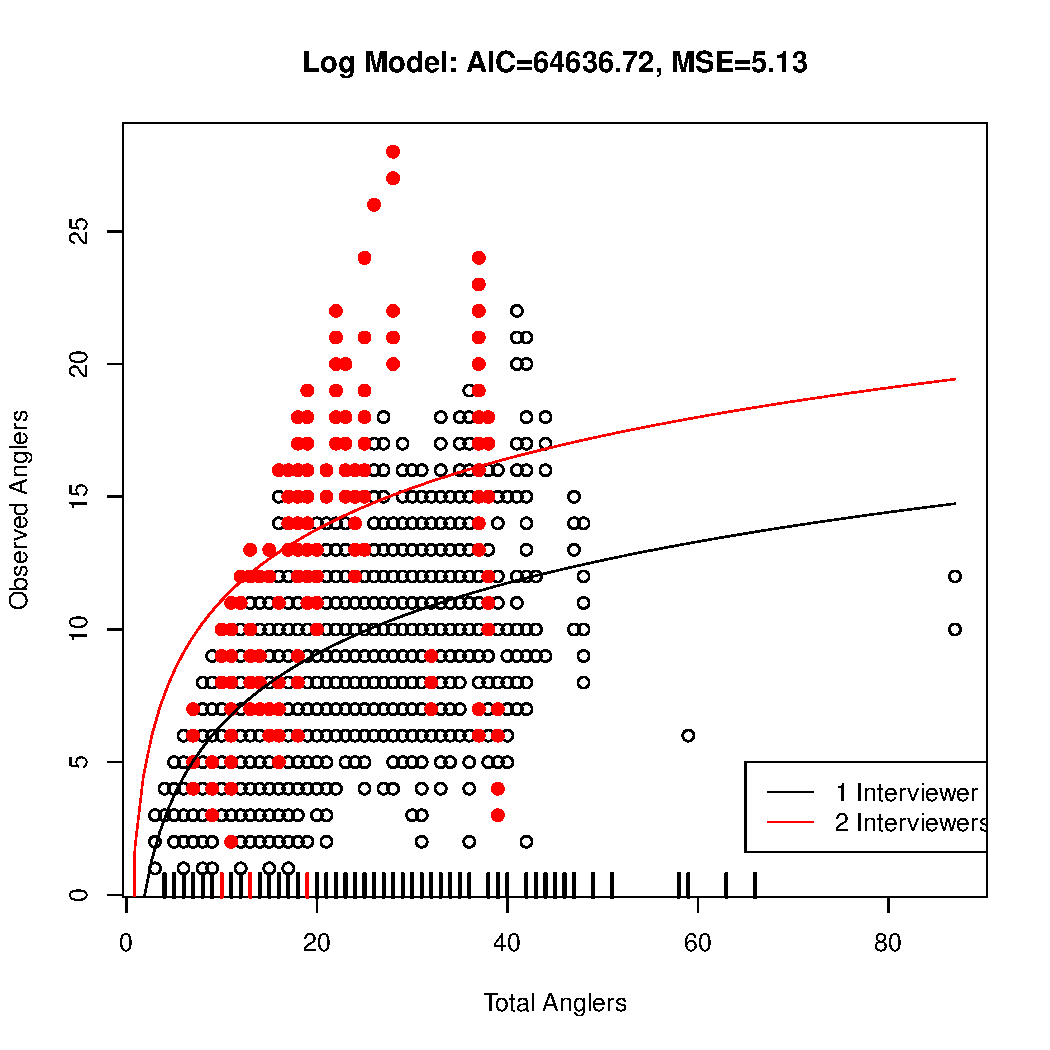
\includegraphics{plots/obsAngLogModel.pdf}
\caption{captions tell all the things \label{obsAngLogModel}}
\end{figure}

Binomial Log Model:

\begin{equation}
y_{ij} \sim B\Big( ~N_{ij}, ~\text{logit}\big(\beta_{0j} + \beta_{1j} \log(x_{ij})\big)~ \Big)
\end{equation}

\begin{figure}[htbp]
\centering
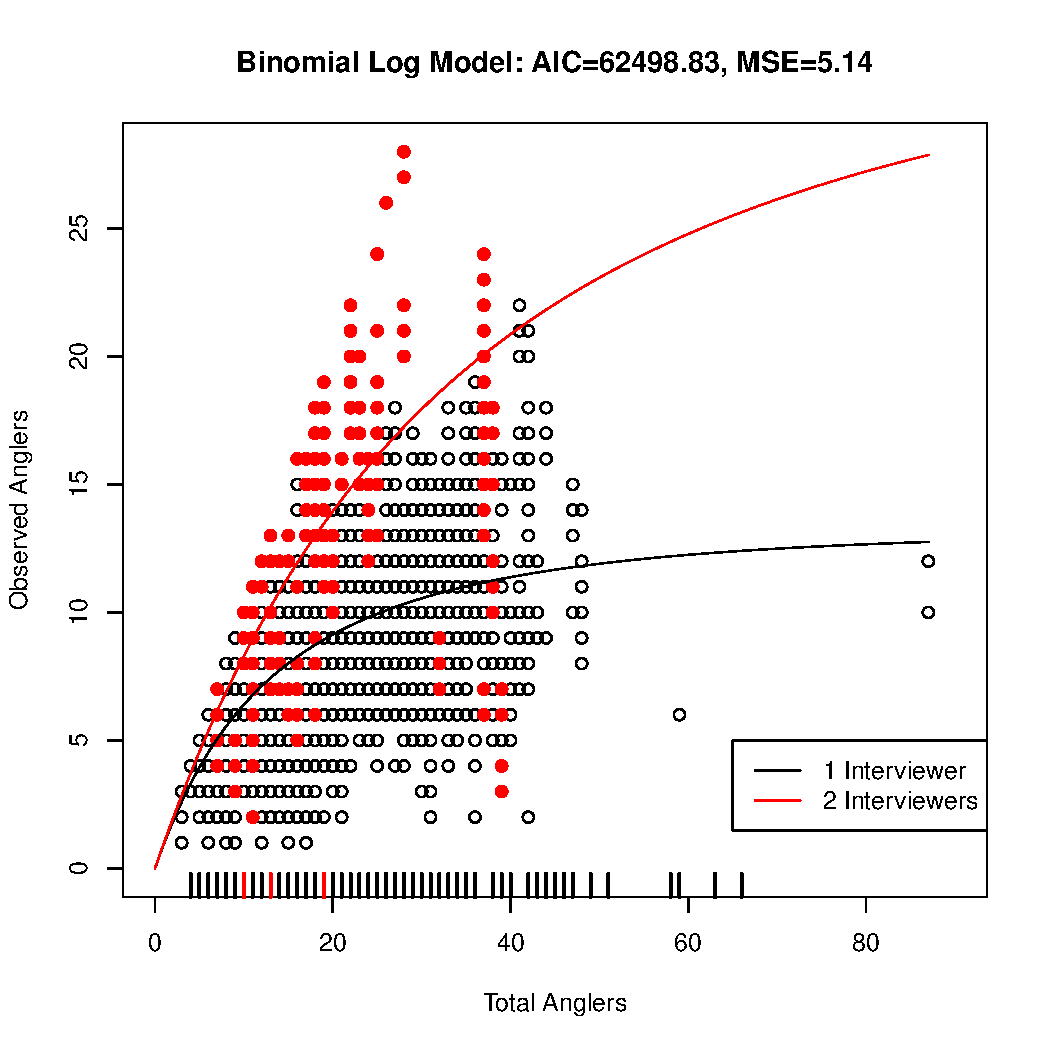
\includegraphics{plots/obsAngGlmLogModel.pdf}
\caption{captions tell all the things \label{obsAngLogModel}}
\end{figure}

\begin{longtable}[c]{@{}cccc@{}}
\toprule
& \verb|totAng| & \verb|totAng + intNum| &
\verb|log(totAng) + intNum|\tabularnewline
\midrule
\endhead
Normal & 67387.29 & 65317.02 & 64636.72\tabularnewline
Binomial & 66099.40 & 63753.06 & 62498.83\tabularnewline
\bottomrule
\end{longtable}

The log model considers a typical normal linear model for each
interviewer level, except it uses the log of the number of total anglers
as a predictor rather than the raw numbers of total anglers. The log
model has several nice features for prediction in this case. Firstly by
regressing on the log of the total anglers it improves the correlation
and relative homoscedasticity of the joint data and improves the
accuracy of sensitivity analysis by improving the standard error
estimates for each parameter. Secondly the log transformation introduces
the expected mean prediction shape, by emphasizing order of magnitude
differences in the total number of anglers. The binomial log model
considers the observed angler counts as independent draws from a
binomial given the know number of total anglers. The log transformation
in the binomial case is justified over the traditional binomial glm for
similar reasons as the normal log model, as well as simple AIC support
of the transformation. All models and model selection criterion were
computed using the standard \verb|glm| function in the R software
environment for statistical computing \cite{rBase}.

The binomial log model was chosen for its low AIC value and reasonable
mean predictions. Untransformed binomial models were considered, however
they produce unreasonable observed angler predictions associated with
the high numbers of total anglers. The log transformed Normal model
provides mostly reasonable predictions, but is not supported by AIC when
compared to the binomial models. Additionally transforms of Normal
likelihood models have no distributional way of producing observed
angler predictions which do not exceed the total number of anglers. If a
Normal likelihood model were to gather AIC support, predictions may
require truncation. These data contain considerable noise, likely due to
the high interviewer turnover rate, which would most effectively be
modeled by including appropriate additional predictors to control for
these effects. At this point no additional predictors from this dataset
were considered to be both sensitive and appropriate for use with
prediction in this case.

\newpage

\thispagestyle{empty} \#References\{-\}

Love, M., Yoklavich, M., and Thorsteinson, L. 2002. The rockfishes of
the northeast Pacific. University of California Press, Berkeley, CA,
USA.

\end{document}
